\subsection{Komplekse egenværdier}
Dette afsnit er baseret på \cite[s.44 - s.xx]{"Morris_and_Stephen"}

\begin{thmx}\textbf{Superpositionsprincippet} \label{sæt:superposition}
\newline
Lad $\frac{d\textbf{x}}{dt}=A\textbf{x}$ være et homogent lineært system. Antag $\textbf{x}_1$ og $\textbf{x}_2$ er løsninger til dette system, og vektorerne $\textbf{x}_1(0)$, $\textbf{x}_2(0)$ er lineært uafhængige. Da gælder det, at
%
\begin{align*}
    \textbf{x}=c_1\textbf{x}_1+c_2\textbf{x}_2
\end{align*}
%
er den entydige løsning til det lineære system, som opfylder $\textbf{x}(0)=c_1\textbf{x}_1(0)+c_2\textbf{x}_2(0)$, hvor $c_1,c_2 \in \R$.
\end{thmx}

\begin{bev}\textbf{}
\newline
Lad $\Phi_1$ og $\Phi_2$ være løsninger til et homogent lineært system, og lad $\Phi_1(0)$ og $\Phi_2(0)$ være lineært uafhængige vektorer. For $c_1,c_2 \in \R$ vil det gælde, at 
%
\begin{align*}
    \frac{d\left(c_1\Phi_1+c_2\Phi_2\right)}{dt} = c_1\frac{d\Phi_1}{dt}+c_2\frac{d\Phi_2}{dt}=c_1A\Phi_1 + c_2A\Phi_2 = A\left(c_1\Phi_2 + c_2\Phi_2\right)
\end{align*}
Da $\Phi(0)$ og $\Phi(0)$ er lineært uafhængige, danner de en basis for løsningsrummet til $x$, hvoraf vektorer udspænder hele løsningsrummet til $x$. Derfor gælder det, at
%
\begin{align*}
    \textbf{x}(0)=c_1\Phi_2(0)+c_2\Phi_2(0)
\end{align*}
%
Dermed er \autoref{sæt:superposition} bevist.
\end{bev}
%
\begin{thmx}\textbf{Komplekse egenværdier}\label{Komplekse_konjugeret_egenværdier_sætning}\\
Lad $\displaystyle\frac{d\textbf{x}}{dt}=\textbf{f(x)}$, hvor $\textbf{f(x)}=A\text{x}$, være et autonomt lineært system. Lad $\lambda = \alpha \pm \beta i$, hvor $\beta \neq 0$, være $A$'s egenværdier. Så gælder der, at hvis
\begin{itemize}
    \item[1.] $\alpha = 0$, så er systemet stabilt;
    \item[2.] $\alpha < 0$, så er systemet asymptotisk stabilt;
    \item[3.] $\alpha > 0$, så er systemet ustabilt.
\end{itemize}
\end{thmx}

\begin{bev} \textbf{}
\newline
Lad følgende begyndelsesværdiproblem være givet det autonome system af første orden differentialligninger.
    \begin{align}
        \frac{d\textbf{x}}{dt}=A\textbf{x}, \quad \textbf{x}(t_0)=0 \label{eq:kompleks_egenværdi_begyndelsesværdiproblem}
    \end{align}
\begin{itemize}
    \item[] \textbf{Bevis for punkt 1}\\
    Antag, at $\alpha = 0$ og $\beta \neq 0$. Da er
    %
    \begin{align*}
        A = \begin{bmatrix}
            \phantom{-}0 & \beta \\
            -\beta & 0
    \end{bmatrix}
    \end{align*}
    %
    Det karakteristiske polynomium kan da udtrykkes ved $\lambda^2+\beta^2=0$. Det bemærkes, at $\beta^2>0$, hvoraf $\lambda=\pm\beta i$. Det ønskes nu at bestemme egenvektoren til $\lambda_1 = \beta i$. Først opstilles det karakteristiske polynomium som et matrixvektor-produkt %ved at løse det karakteristiske polynomium $(A-\lambda I)\textbf{v}=\textbf{0}$.
    %
    \begin{align*}
        \begin{bmatrix}
            -\beta i & \phantom{-}\beta \\
            -\beta & -\beta i 
        \end{bmatrix}
        \begin{bmatrix}
            x_1 \\ x_2
        \end{bmatrix}
        =
        \textbf{0}
    \end{align*}
    %
    Herefter bestemmes egenvektoren ved at løse $\beta i x_1=\beta x_2$. Herved bestemmes egenvektoren til $\lambda_1$ til at være $v=\begin{bmatrix} 1 & i\end{bmatrix}^T$. Herefter anvendes \autoref{sæt:Løsning_for_komplekse_egenværdier} til at bestemme en løsning til \eqref{eq:kompleks_egenværdi_begyndelsesværdiproblem}.
    %
    \begin{align} \label{eq:kompleks_egenværdi_bevis_1}
        \frac{d\textbf{x}}{dt}=e^{t\beta i}\begin{bmatrix} 1 \\ i \end{bmatrix}
    \end{align}
    %  
    Euler's formel anvendes til at omskrive $e^{t\beta i}$.
    %
    \begin{align} \label{eq:kompleks_egenværdi_bevis_2}
        e^{t\beta i} = \cos(t \beta) + \sin(t \beta) i
    \end{align}
    %
    \eqref{eq:kompleks_egenværdi_bevis_2} indsættes i \eqref{eq:kompleks_egenværdi_bevis_1}
    %
    \begin{align*}
        \frac{d\textbf{x}}{dt}=  \left(\cos(t \beta) + \sin(t \beta )i\right)\begin{bmatrix} 1 \\ i \end{bmatrix} = \begin{bmatrix} \phantom{-}\cos(t \beta) + \sin(t \beta)i \\ - \sin(t \beta) + \cos(t \beta)i \end{bmatrix}
    \end{align*}
    %
    Herefter opdeles systemet i den reelle og imaginære del
    %
    \begin{align*}
        \frac{d\textbf{x}}{dt}&=\text{Re}\left(\textbf{x}\right) +\text{Im}\left(\textbf{x}\right)i \\
        &\Uptown \\
        \frac{d\textbf{x}}{dt} &= \begin{bmatrix} \phantom{-}\cos(t \beta) \\ - \sin(t \beta) \end{bmatrix} + \begin{bmatrix} \sin(t \beta) \\ \cos(t \beta) \end{bmatrix}i
    \end{align*}
    %
    Det bemærkes, at både den reelle og imaginære del er løsninger til det oprindelige begyndelsesværdiproblem \eqref{eq:kompleks_egenværdi_begyndelsesværdiproblem}. 
    %
    \begin{align*}
        \frac{d\big(\text{Re}\left(\textbf{x}\right)\big)}{dt} + \frac{d\big(\text{Im}\left(\textbf{x}\right)\big)}{dt}i &= \frac{d\textbf{x}}{dt} \\
        &= A\textbf{x} \\
        &= A\left(\text{Re}\left(\textbf{x}\right) + \text{Im}\left(\textbf{x}\right)i\right) \\
        &= A\cdot\text{Re}\left(\textbf{x}\right) + A\cdot\text{Im}\left(\textbf{x}\right)i
    \end{align*}
    %
    Ovenstående lighed giver følgende første ordens autonome differentialligninger
    %
    \begin{align*}
        \frac{d\left(\text{Re}\left(\textbf{x}\right)\right)}{dt} = A\cdot\text{Re}\left(\textbf{x}\right) , \quad
        \frac{d\left(\text{Im}\left(\textbf{x}\right)\right)}{dt} = A\cdot\text{Im}\left(\textbf{x}\right)
    \end{align*}
    %
    Derudover gælder det, at
    %
    \begin{align*}
        \text{Re}\left(\textbf{x}(0)\right) = \begin{bmatrix} \phantom{-}\cos(0) \\
        -\sin(0) \end{bmatrix} = \begin{bmatrix} 1 \\
        0 \end{bmatrix}, \quad
        \text{Im}\left(\textbf{x}(0)\right) = \begin{bmatrix} \sin(0) \\
        \cos(0) \end{bmatrix} = \begin{bmatrix} 0 \\
        1 \end{bmatrix} 
    \end{align*}
    %
    Ud fra ovenstående vektorer bemærkes det, at de to løsninger er lineært uafhængige. Jævnfør \autoref{sæt:superposition}, kan den generelle løsning til \eqref{eq:kompleks_egenværdi_begyndelsesværdiproblem} opskrives således
    %
    \begin{align} \label{eq:kompleks_egenværdier_bevis_generel_løsning}
        \textbf{x} = c_1\begin{bmatrix} \phantom{-}\cos(t\beta) \\
        -\sin(t\beta) \end{bmatrix} + c_2\begin{bmatrix} \sin(t\beta) \\
        \cos(t\beta) \end{bmatrix}
    \end{align}
    hvor $c_1,c_2 \in \R$. Ud fra eksistens- og entydighedssætningen, \autoref{sæt:eksistens_og_entydighed}, og \eqref{eq:kompleks_egenværdier_bevis_generel_løsning} kan man bestemme den entydige løsning for enhver begyndelsesbetingelse. Det bemærkes, at den generelle løsning er periodisk funktion med perioden $\frac{2\pi}{\beta}$. Dette betyder, at for enhver begyndelsesbetingelse vil løsningskurven være en cirkel omkring ligevægtspunktet $\textbf{x}^*$ for $t \to \infty$. For $\beta>0$, vil banen bevæge sig højre om ligevægtspunktet, og for $\beta<0$, vil banen bevæge sig venstre om ligevægtspunktet. Dette er illustreret nedenfor.
    
    \textbf{indsæt sejt billede af tilfælde?????????????} Vær' så god
    
    \begin{minipage}{0.4\textwidth}
    \begin{figure}[H]
        \centering
        \captionsetup{justification=centering}
        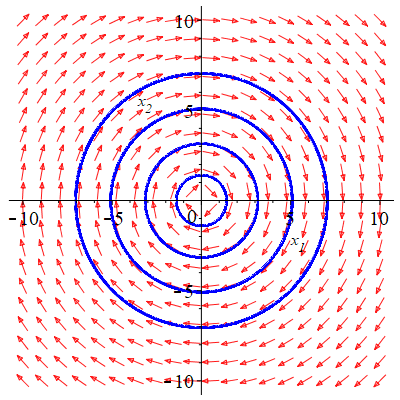
\includegraphics[scale=0.4]{Billeder/spiral_alpha_eq_0_beta_geq_0.png}
        \caption{Fasediagram for $\alpha=0$ og $\beta>0$}
        \label{fig:fase_komplekse_egenværdier_alpha_eq_0_beta_geq_0}
    \end{figure}
    \end{minipage}
    \hfill
    \begin{minipage}{0.4\textwidth}
    \begin{figure}[H]
        \centering
        \captionsetup{justification=centering}
        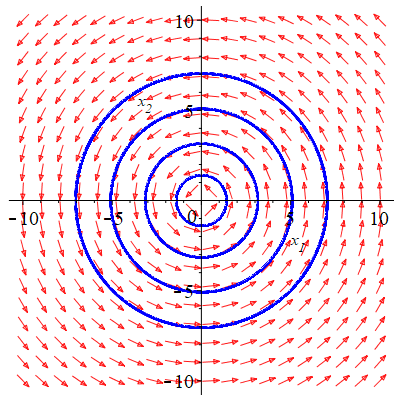
\includegraphics[scale=0.4]{Billeder/spiral_alpha_eq_0_beta_leq_0.png}
        \caption{Fasediagram for $\alpha=0$ og $\beta<0$}
        \label{fig:fase_komplekse_egenværdier_alpha_eq_0_beta_leq_0}
    \end{figure}
    \end{minipage}
    
    Dermed er det bevist, at når $\alpha=0$ vil det autonome system af første ordens differentialligninger være stabilt for $t \to \infty$.
    
    \item[] \textbf{Bevis for punkt 2 og punkt 3}\\
    Antag, at $\alpha,\beta \neq 0$. Da er 
    %
    \begin{align*}
        A = \begin{bmatrix}
            \alpha & \beta \\
            -\beta & \alpha
            \end{bmatrix}
    \end{align*}
    Det karakteristiske polynomium kan da udtrykkes ved $\lambda^2-2\alpha\lambda+\alpha^2+\beta^2$, så egenværdierne til $A$ kan bestemmes ved $\lambda = \alpha \pm \beta i$. Egenvektoren til $\lambda_1 = \alpha + \beta i$ bestemmes efter samme fremgangsmåde som i beviset, hvor $\alpha = 0$.
    %
    \begin{align*}
        \left(\alpha-(\alpha + \beta i)x_1\right) + \beta x_2 = 0
    \end{align*}
    %
    Egenvektoren til $\lambda_1$ bestemmes igen til at være $\textbf{v}=\begin{bmatrix} 1 & i\end{bmatrix}^T$. Herefter anvendes \autoref{sæt:Løsning_for_komplekse_egenværdier} til at bestemme en løsning til \eqref{eq:kompleks_egenværdi_begyndelsesværdiproblem}. 
    %
    \begin{align} \label{eq:komplekse_egenværdier_bevis2_1}
        \frac{d\textbf{x}}{dt}&=e^{t(\alpha+\beta i)}\begin{bmatrix}
            1 \\ i
        \end{bmatrix} 
    \end{align}
   %
   Eulers formel anvendes til at omskrive $e^{(\alpha+\beta i)t}$
   %
   \begin{align} \label{eq:komplekse_egenværdier_bevis2_2}
       e^{t(\alpha+\beta i)} = e^{t\alpha}e^{t\beta i }=e^{t\alpha }\left(\cos(t\beta ) + \sin(t\beta)i \right)
   \end{align}
   %
   \eqref{eq:komplekse_egenværdier_bevis2_2} indsættes \eqref{eq:komplekse_egenværdier_bevis2_1}.
   %
   \begin{align*}
       \frac{d\textbf{x}}{dt}&=e^{t\alpha}
       \begin{bmatrix}
           \phantom{-}\cos(t\beta) \\ -sin(t\beta)
       \end{bmatrix}
       + e^{t\alpha} 
       \begin{bmatrix}
           \sin(t\beta) \\ \cos(t\beta)
       \end{bmatrix}i \\
       &= \text{Re}(\textbf{x}) + \text{Im}(\textbf{x})i
   \end{align*}
   %
   Med samme fremgangsmåde som i beviset, hvor $\alpha = 0$, bestemmes Re$(\textbf{x})$ og Im$(\textbf{x})$ til at være reelle løsninger, som er lineært uafhængige. Herefter bestemmes den generelle løsning til \eqref{eq:kompleks_egenværdi_begyndelsesværdiproblem} jævnfør \autoref{sæt:superposition}.
   %
   \begin{align} \label{eq:komplekse_egenværdier_generel_løsning2}
       \textbf{x} = c_1e^{t\alpha}
       \begin{bmatrix}
           \phantom{-}\cos(t\beta) \\ -sin(t\beta)
       \end{bmatrix}
       + c_2e^{t\alpha} 
       \begin{bmatrix}
           \sin(t\beta) \\ \cos(t\beta)
       \end{bmatrix} 
   \end{align}
   %
   hvor $c_1,c_2 \in \R$. Ud fra eksistens- og entydighedssætningen, \autoref{sæt:eksistens_og_entydighed}, og \eqref{eq:komplekse_egenværdier_generel_løsning2} kan man bestemme den entydige løsning for enhver begyndelsesbetingelse. Det bemærkes, at uden $e^{\alpha t}$-ledende, vil løsningen være identisk med \eqref{eq:kompleks_egenværdier_bevis_generel_løsning}. Derudover bemærkes det, at hvis $\alpha<0$, vil $e^{t\alpha} \to 0$ for $t \to \infty$, hvoraf systemet er asymptotisk stabilt. For $\alpha>0$ vil $e^{t\alpha} \to \infty$ for $t \to \infty$, hvoraf systemet er ustabilt.
   
   \textbf{sejt bette billed af tilfælde??????????}
   \textbf{Værsgo, håber du nyder det}
   
   \begin{minipage}{0.4\textwidth}
   \begin{figure}[H]
       \centering
       \captionsetup{justification=centering}
       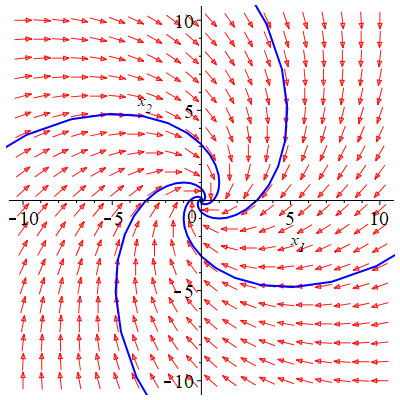
\includegraphics[scale=0.4]{Billeder/spiral_alpha_leq_0.png}
       \caption{Fasediagram for $\alpha<0$.}
       \label{fig:fase_komplekse_egenværdier_alpha_leq_0}
   \end{figure}
   \end{minipage}
   \hfill
   \begin{minipage}{0.4\textwidth}
   \begin{figure}[H]
       \centering
       \captionsetup{justification=centering}
       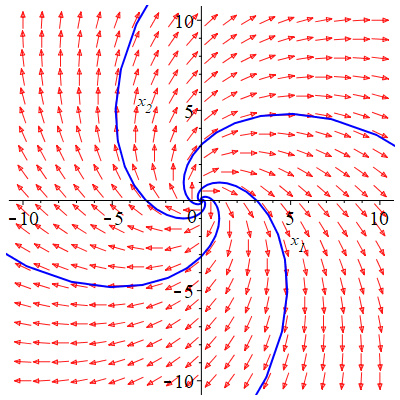
\includegraphics[scale=0.4]{Billeder/spiral_alpha_geq_0.png}
       \caption{Fasediagram for $\alpha>0$.}
       \label{fig:fase_komplekse_egenværdier_alpha_geq_0}
   \end{figure}
   \end{minipage}
\end{itemize}
Dermed er \autoref{Komplekse_konjugeret_egenværdier_sætning} bevist.
\end{bev}